\documentclass[11pt, a4paper]{article}
\usepackage[dutch, english]{babel}
\usepackage[pdftex]{graphicx}
\usepackage[linkcolor=black,urlcolor=black,citecolor=black]{hyperref}
\usepackage[font=small,format=plain,labelfont=bf,up,textfont=it,up]{caption}
\usepackage[usenames,dvipsnames]{pstricks}
\usepackage{epsfig}
\usepackage[parfill]{parskip}
\hypersetup{colorlinks=true}
\usepackage{amsmath, epic, eepic, float, subfig, amsfonts, color, amsthm,xfrac,textcomp}
\usepackage[all]{xy}
\newcommand{\HRule}{\rule{\linewidth}{0.5mm}}
\DeclareMathOperator{\bgtan}{bgtan}




\begin{document}




\selectlanguage{dutch}
\begin{titlepage}
\begin{center}

\includegraphics[width=0.5\textwidth]{./IMG/logo}~\\[1cm]



% Vak
\textsc{\Large Labo Linux}\\[0.5cm]


% Titel
\HRule \\[0.4cm]
{ \LARGE \bfseries Installatie Ubuntu}\\[0.4cm]
{\large \em{project 1}}\\[0.2cm]




\HRule \\[1.5cm]

% Door en jaar
\begin{minipage}{0.4\textwidth}
\begin{flushleft} \large
\emph{Door:}\\
Haroen \textsc{Viaene}\\
\ \ \ \ \ \ \ \ \ \,r0457976\\
\end{flushleft}
\end{minipage}
\begin{minipage}{0.4\textwidth}
\begin{flushright} \large
\large{1$^{\text{ste}}$ fase bachelor electronica-ICT}\\
\end{flushright}
\end{minipage}





\vfill

% Jaar
{\large 2014-2014}



\end{center}
\end{titlepage}







\newpage


% Inhoud
\section{Inhoud}
\tableofcontents

\newpage




\section{Doelstelling}
Het doel is om Ubuntu te installeren op een installatie van DOS, die later nog steeds bruikbaar moet zijn. Ik heb VirtualBox gebruikt, en ik heb gemerkt dat de inhoud van het .vmx-bestand niet veranderd is voor en na het opstarten, installeren en gebruiken van Ubuntu. Ik heb het daarom niet bijgevoegd.




\section{Installatie van Ubuntu}

Eerst wordt DOS opgestart in VirtualBox. Dit doen we door de .vmdk te openen die op Toledo te vinden is. 

\begin{figure}[H]
	\centering
	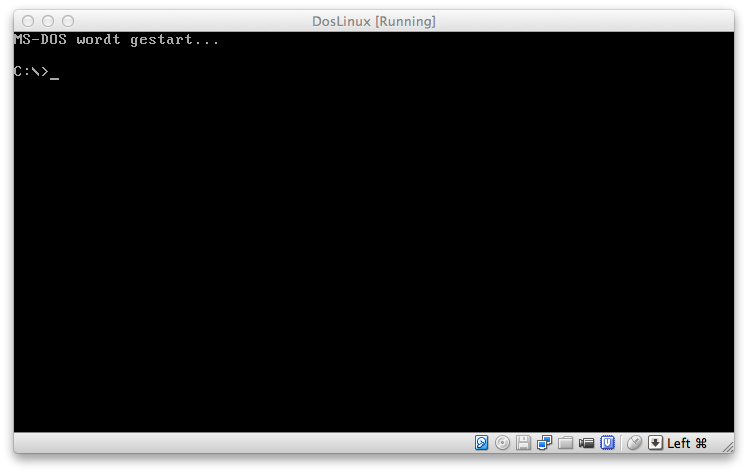
\includegraphics[width=\textwidth]{./IMG/A}
	\caption{DOS-Venster}
\end{figure}

In DOS wordt de vrije ruimte bekeken met 'fdisk'

\begin{figure}[H]
	\centering
	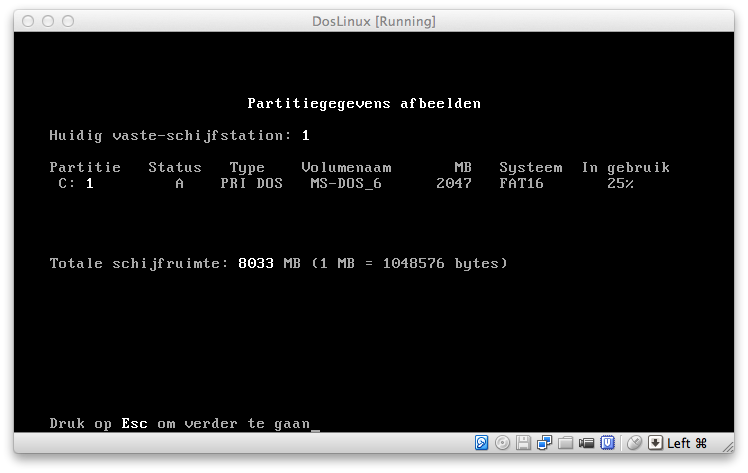
\includegraphics[width=\textwidth]{./IMG/B}
	\caption{fdisk}
\end{figure}

Dan wordt de live-cd van Ubuntu gekoppeld: 

\begin{figure}[H]
	\centering
	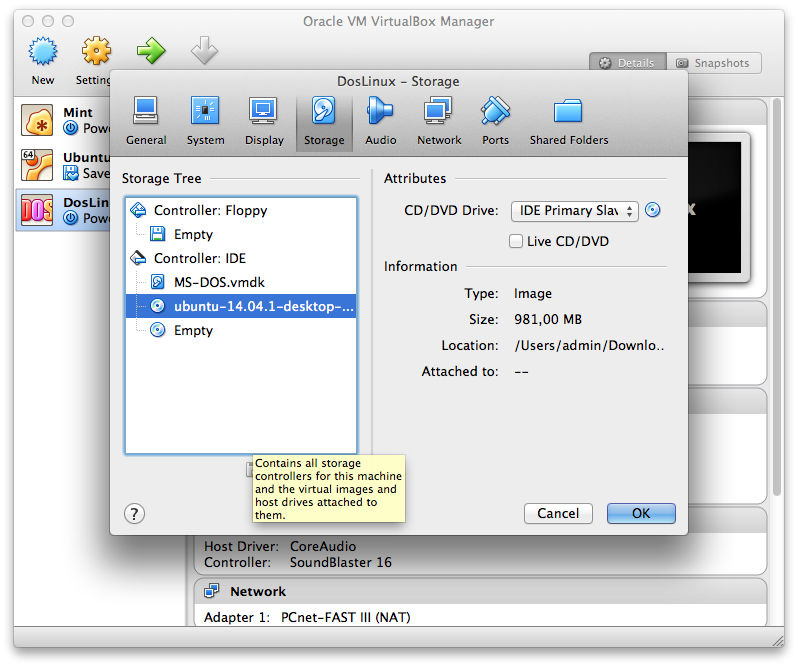
\includegraphics[width=\textwidth]{./IMG/C}
	\caption{VirtualBox instellingen}
\end{figure}

Hierna start Ubuntu op:

\begin{figure}[H]
	\centering
	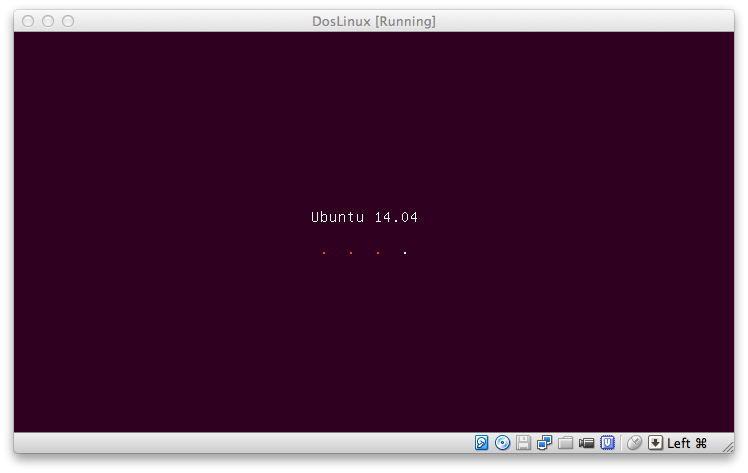
\includegraphics[width=\textwidth]{./IMG/D}
\end{figure}

\begin{figure}[H]
	\centering
	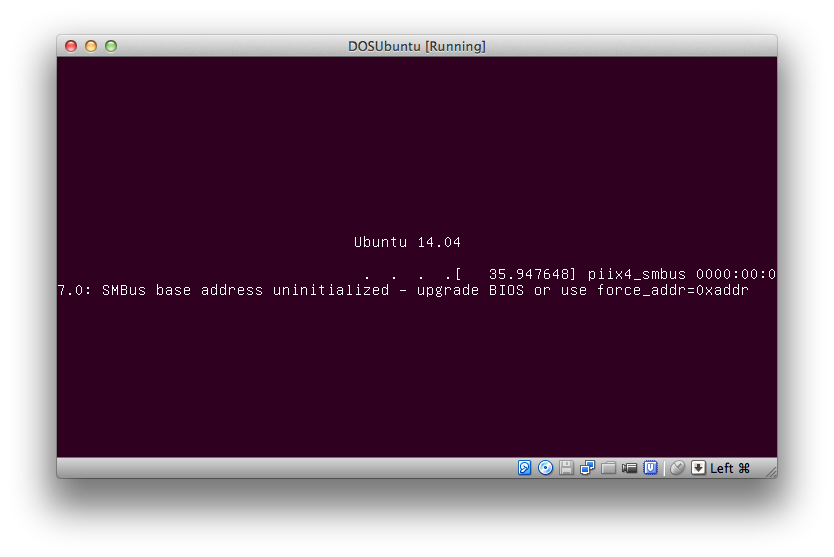
\includegraphics[width=\textwidth]{./IMG/E}
\end{figure}

\begin{figure}[H]
	\centering
	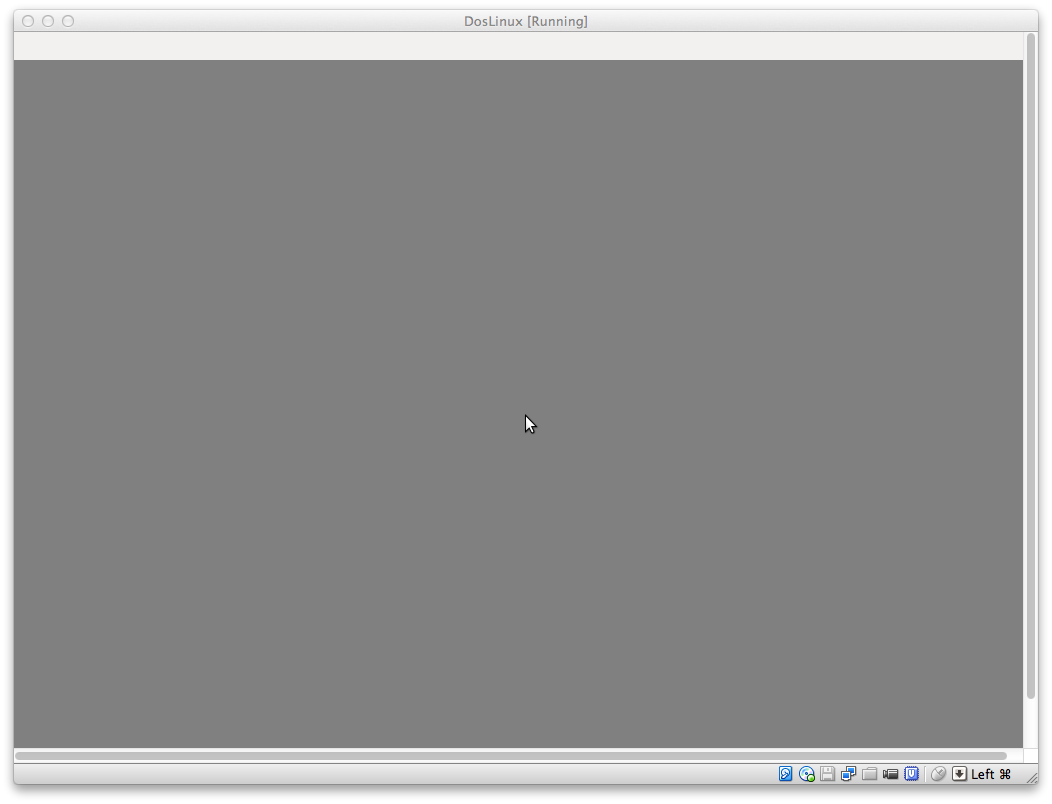
\includegraphics[width=\textwidth]{./IMG/F}
\end{figure}

\begin{figure}[H]
	\centering
	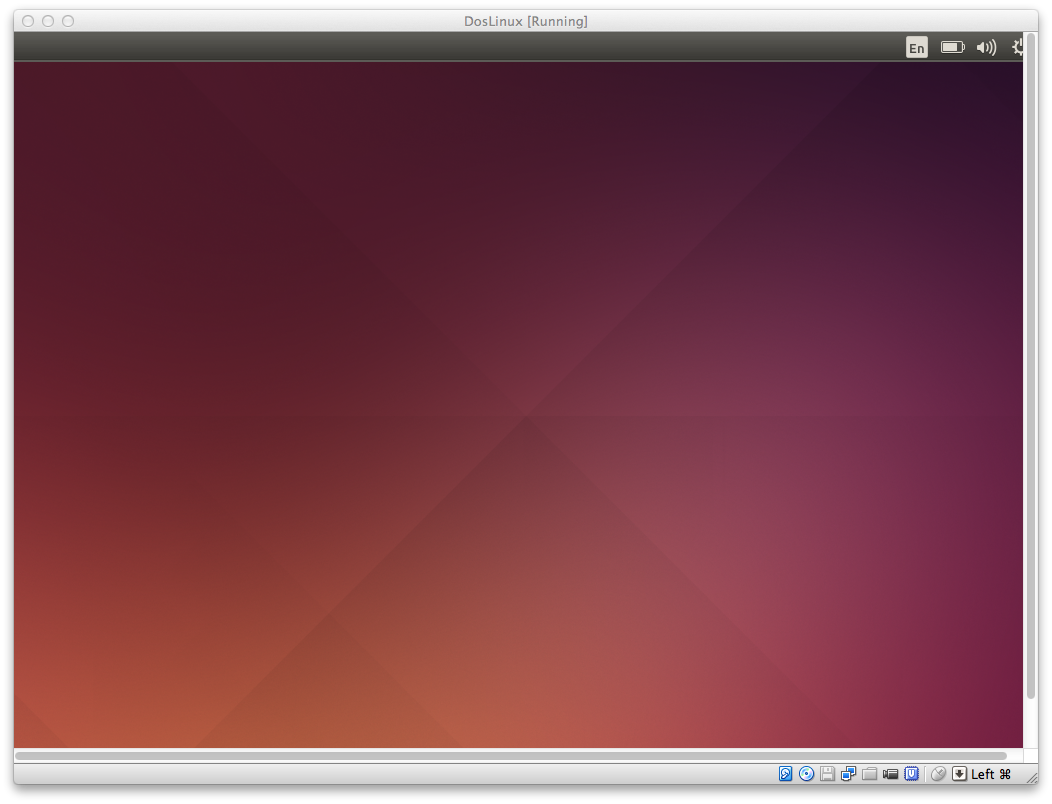
\includegraphics[width=\textwidth]{./IMG/G}
\end{figure}

Nu kan Ubuntu echt ge\"installeerd worden.

\begin{figure}[H]
	\centering
	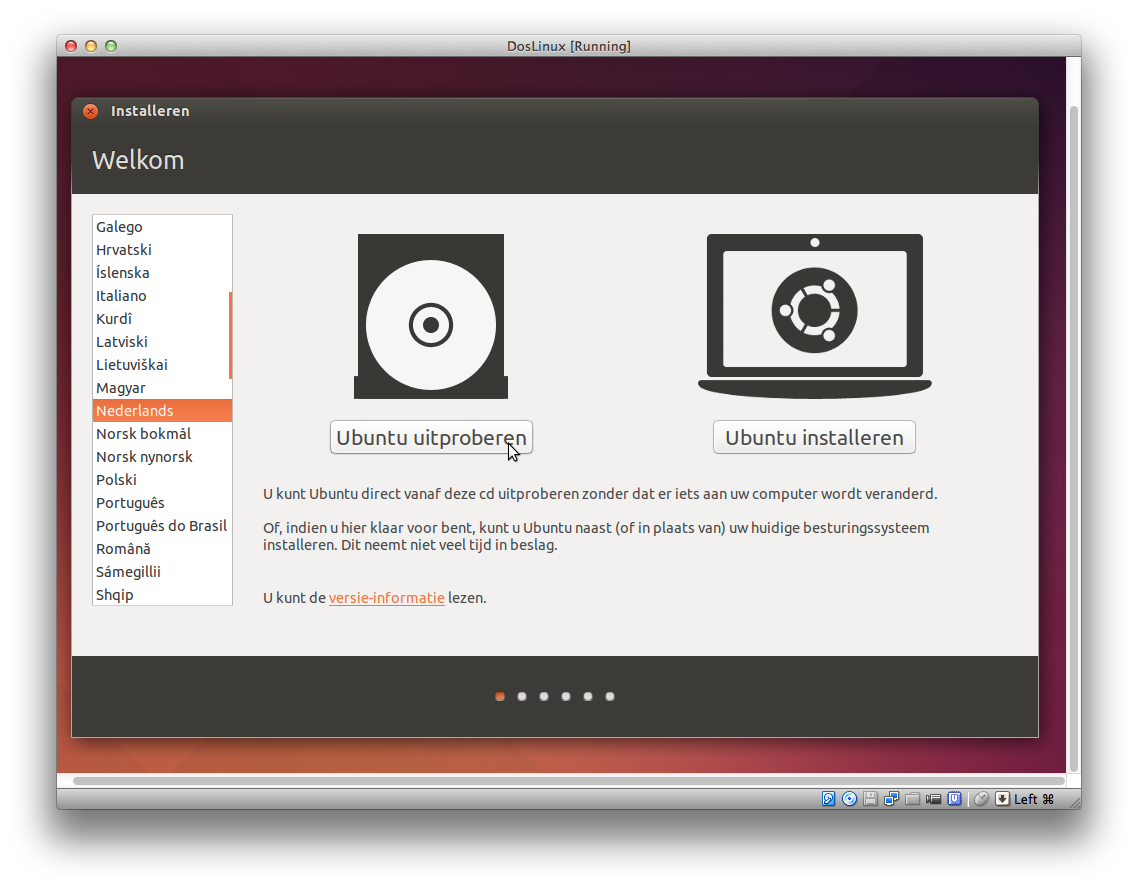
\includegraphics[width=\textwidth]{./IMG/H}
\end{figure}

\begin{figure}[H]
	\centering
	
\includegraphics[width=\textwidth]{./IMG/I}
\end{figure}

\begin{figure}[H]
	\centering
	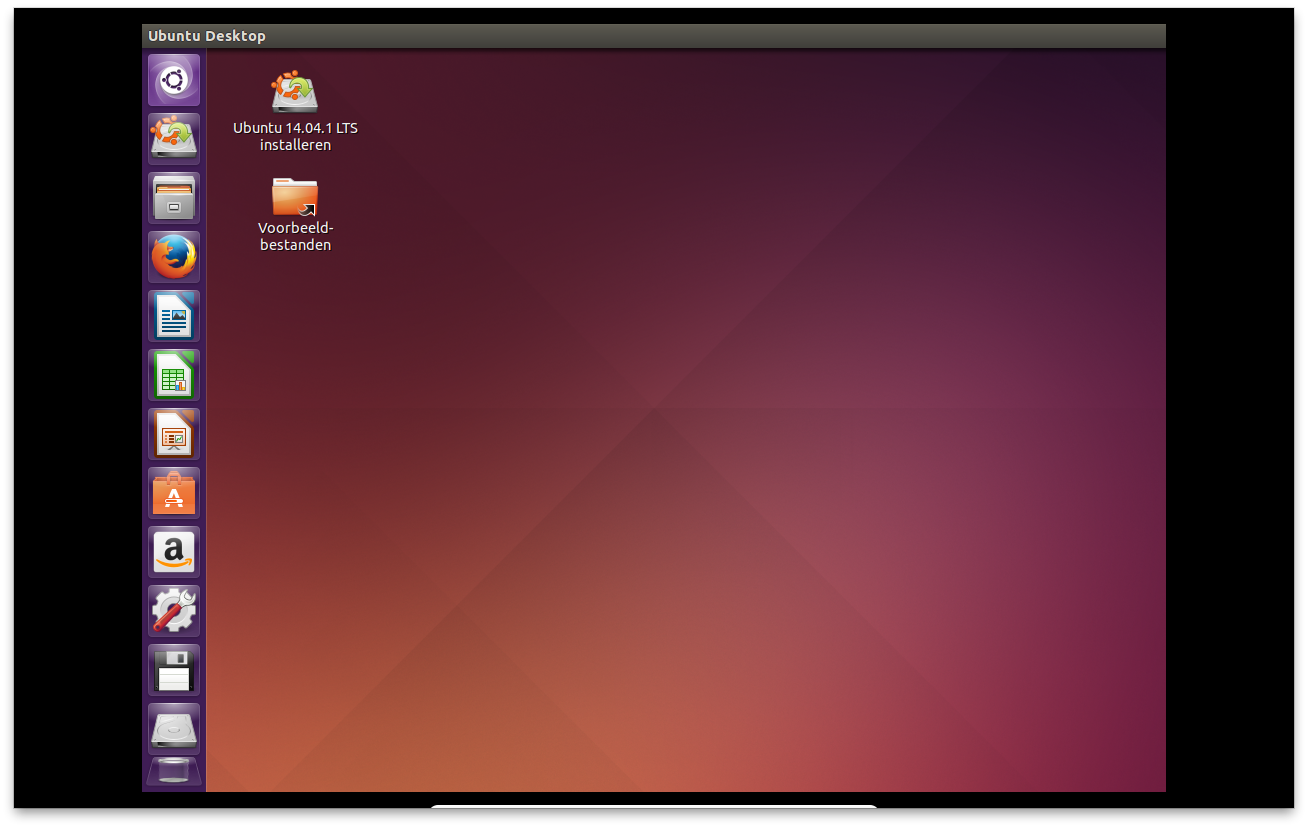
\includegraphics[width=\textwidth]{./IMG/J}
\end{figure}

\begin{figure}[H]
	\centering
	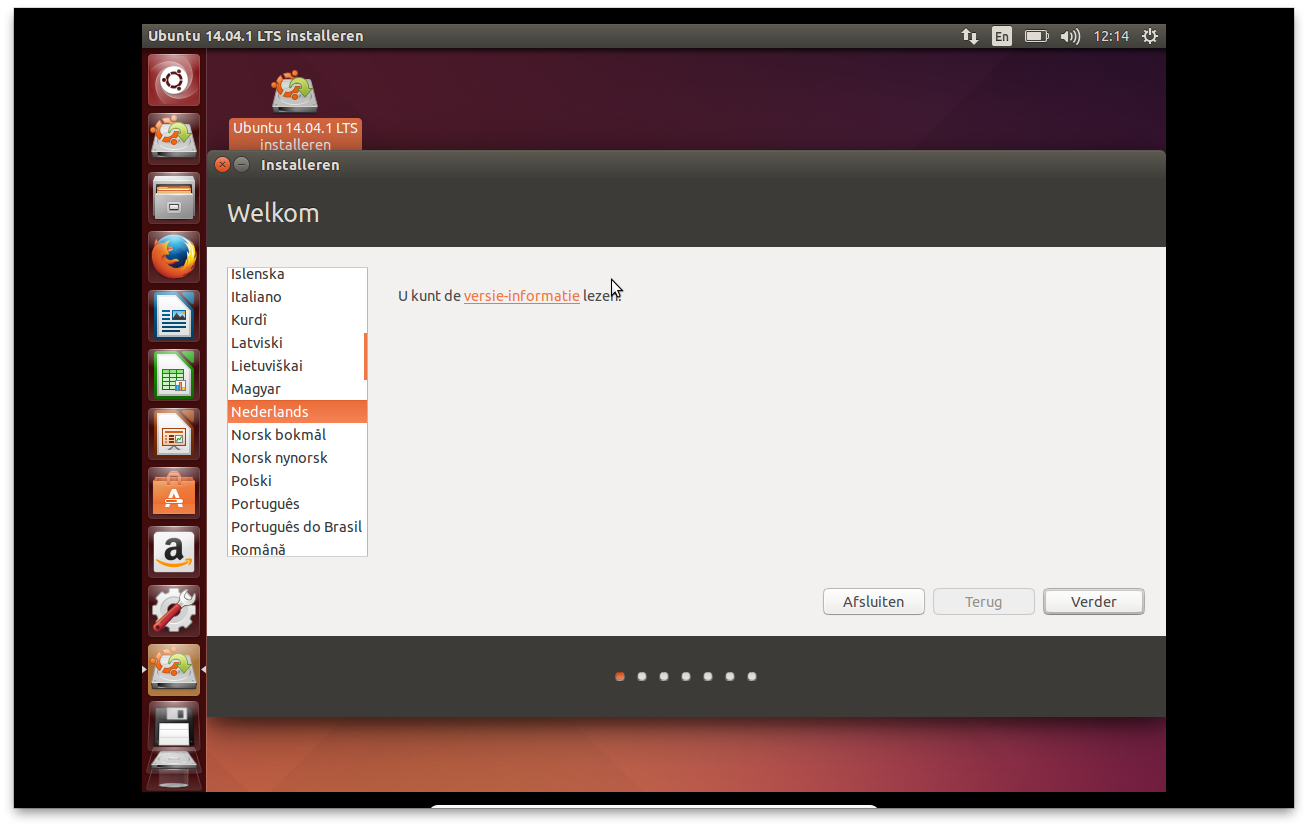
\includegraphics[width=\textwidth]{./IMG/K}
\end{figure}

\begin{figure}[H]
	\centering
	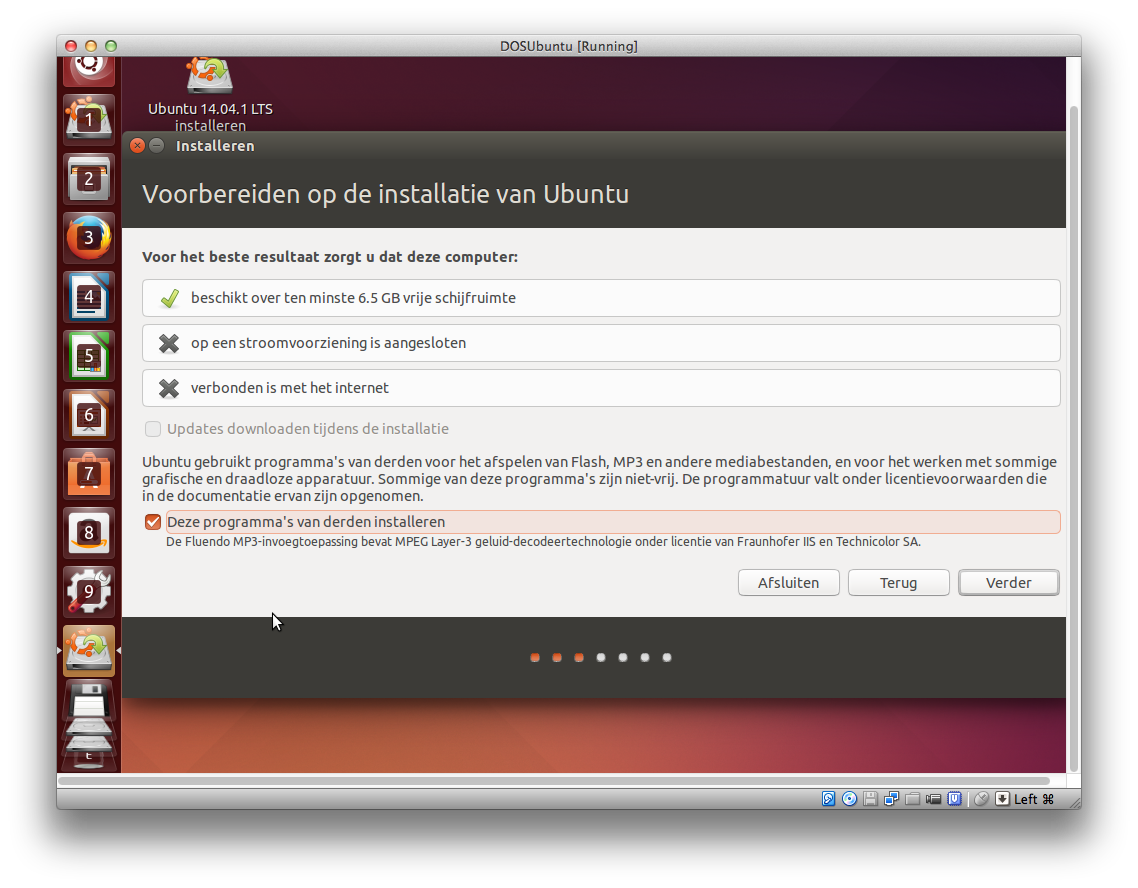
\includegraphics[width=\textwidth]{./IMG/L}
\end{figure}

\begin{figure}[H]
	\centering
	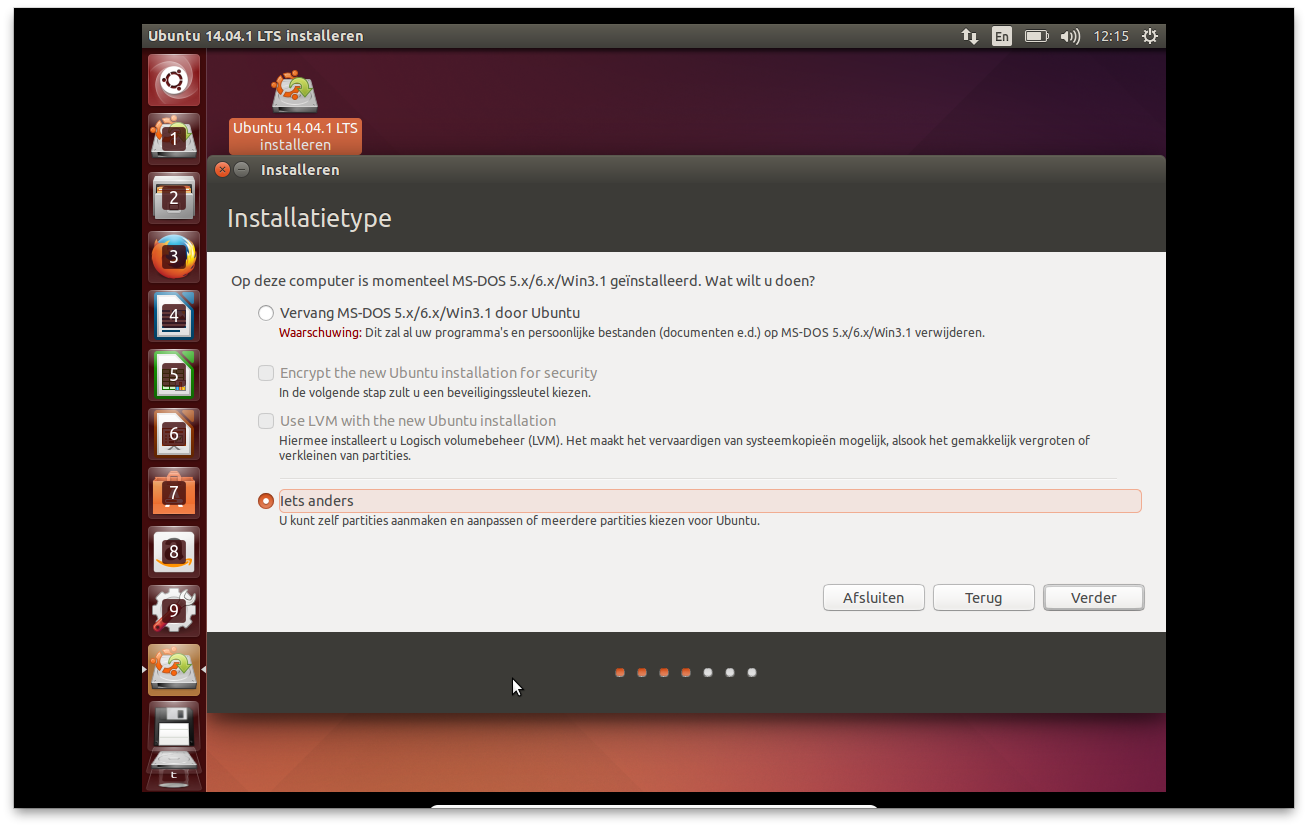
\includegraphics[width=\textwidth]{./IMG/M}
\end{figure}

\begin{figure}[H]
	\centering
	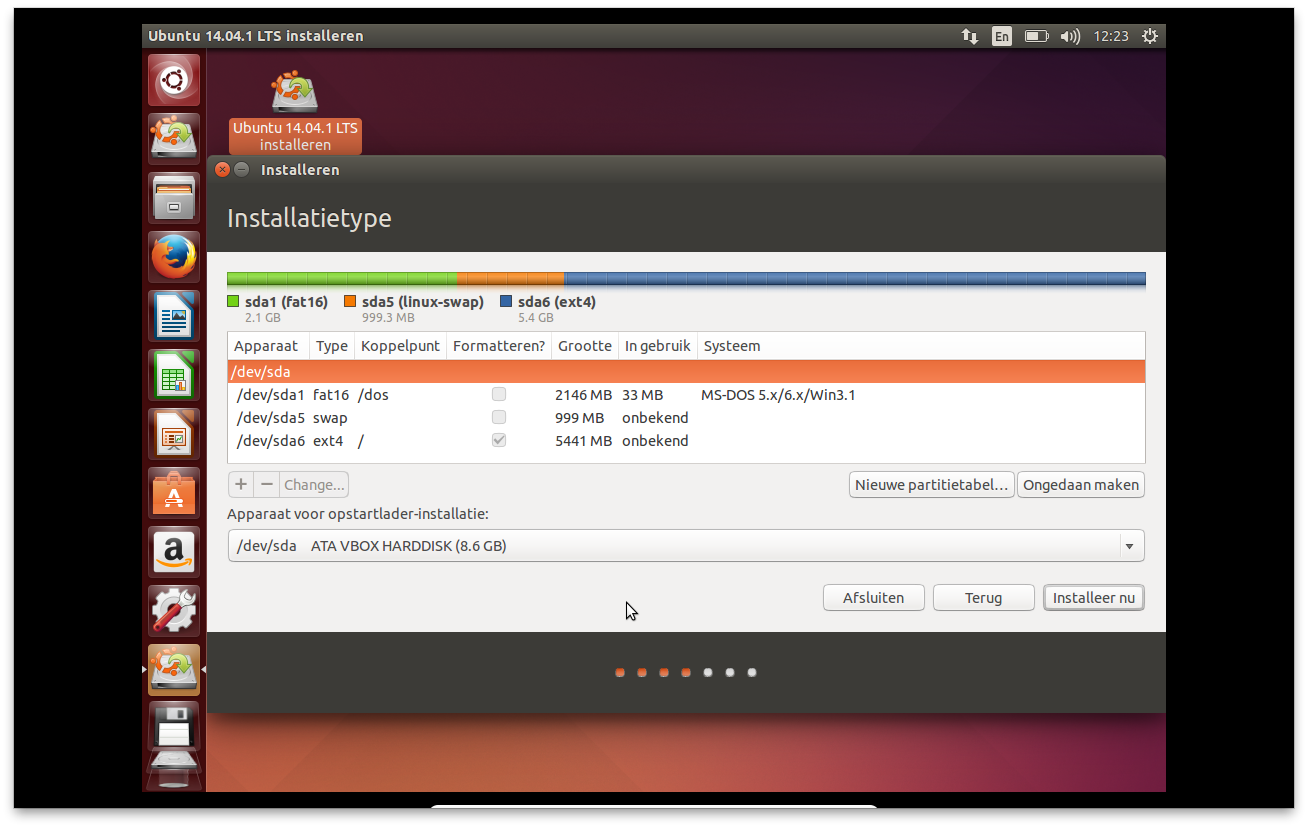
\includegraphics[width=\textwidth]{./IMG/N}
\end{figure}

\begin{figure}[H]
	\centering
	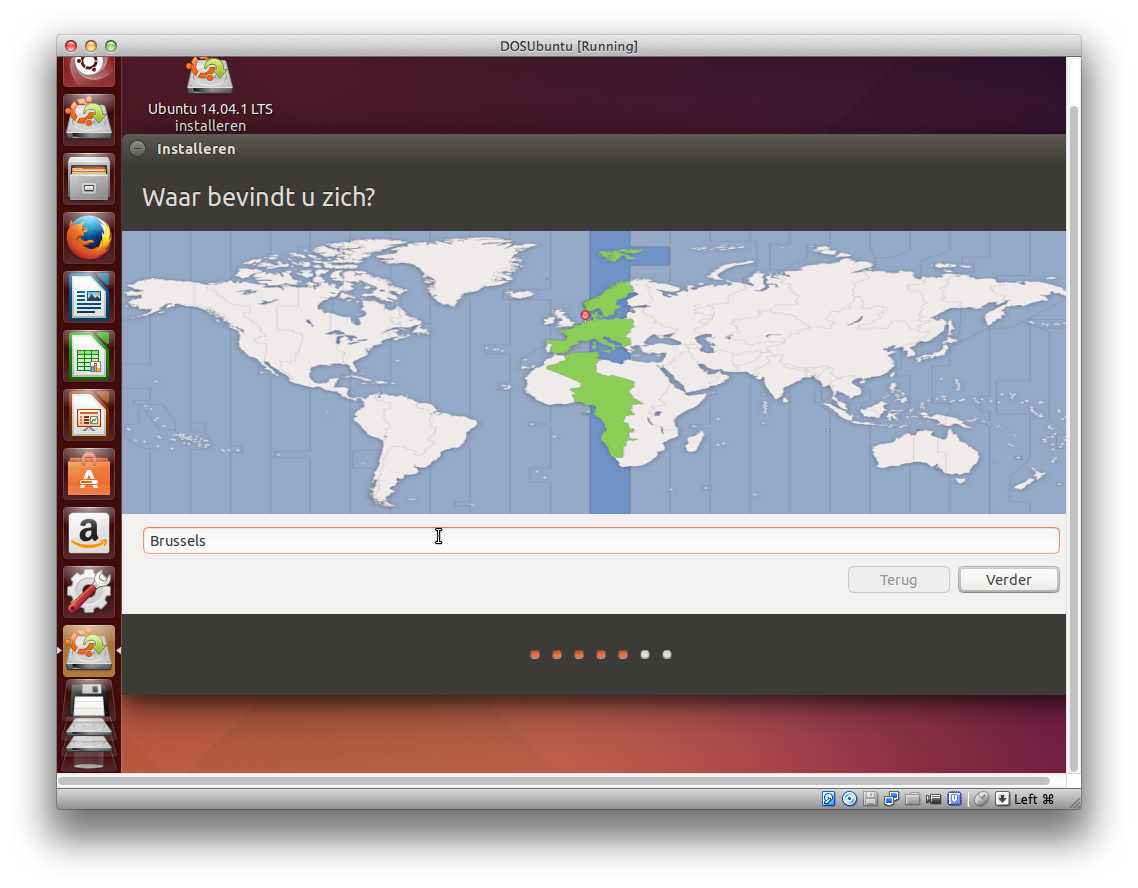
\includegraphics[width=\textwidth]{./IMG/O}
\end{figure}

\begin{figure}[H]
	\centering
	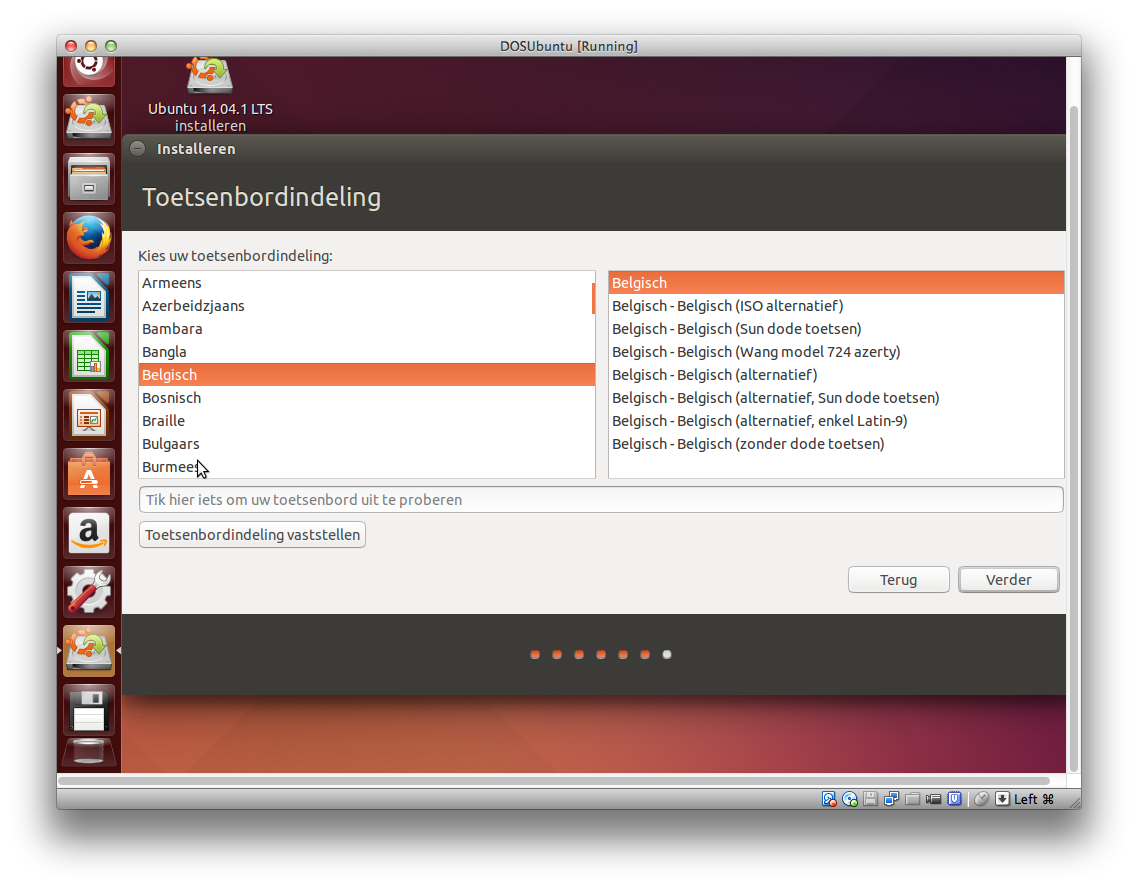
\includegraphics[width=\textwidth]{./IMG/P}
\end{figure}

\begin{figure}[H]
	\centering
	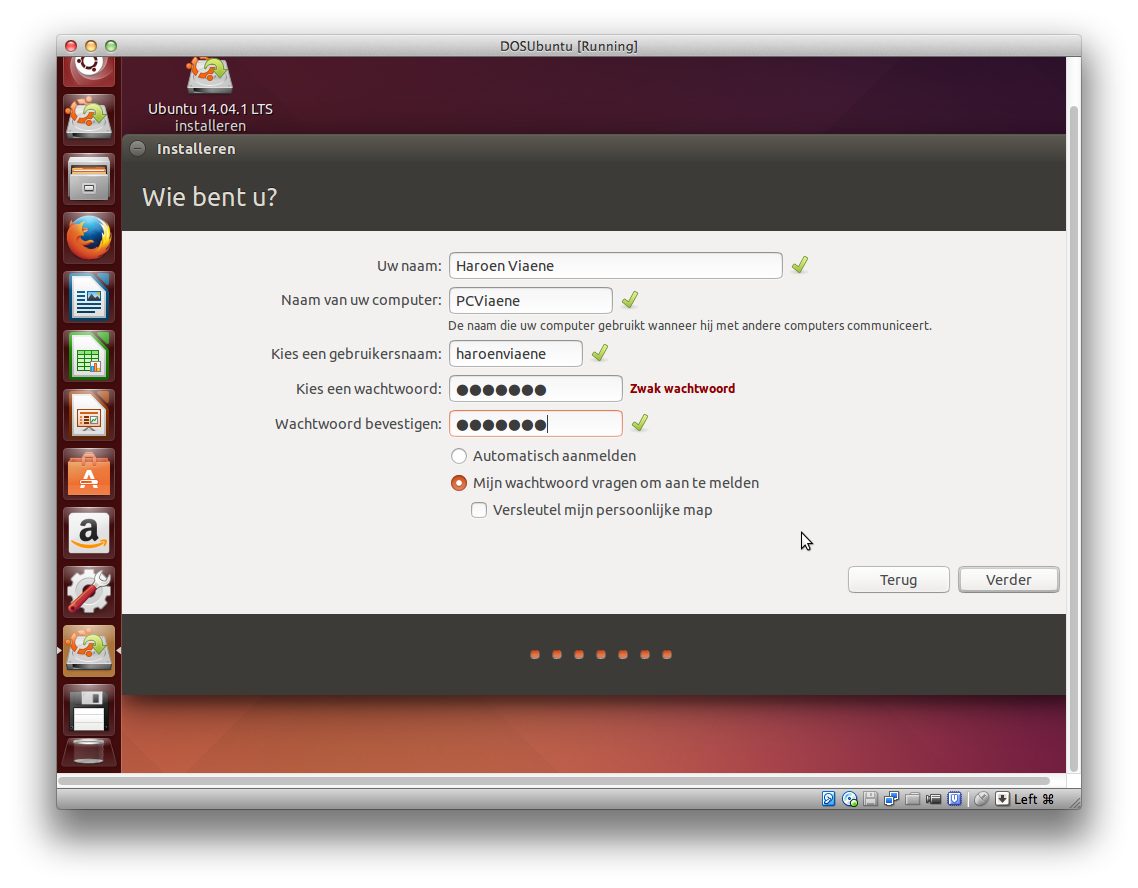
\includegraphics[width=\textwidth]{./IMG/Q}
\end{figure}

\begin{figure}[H]
	\centering
	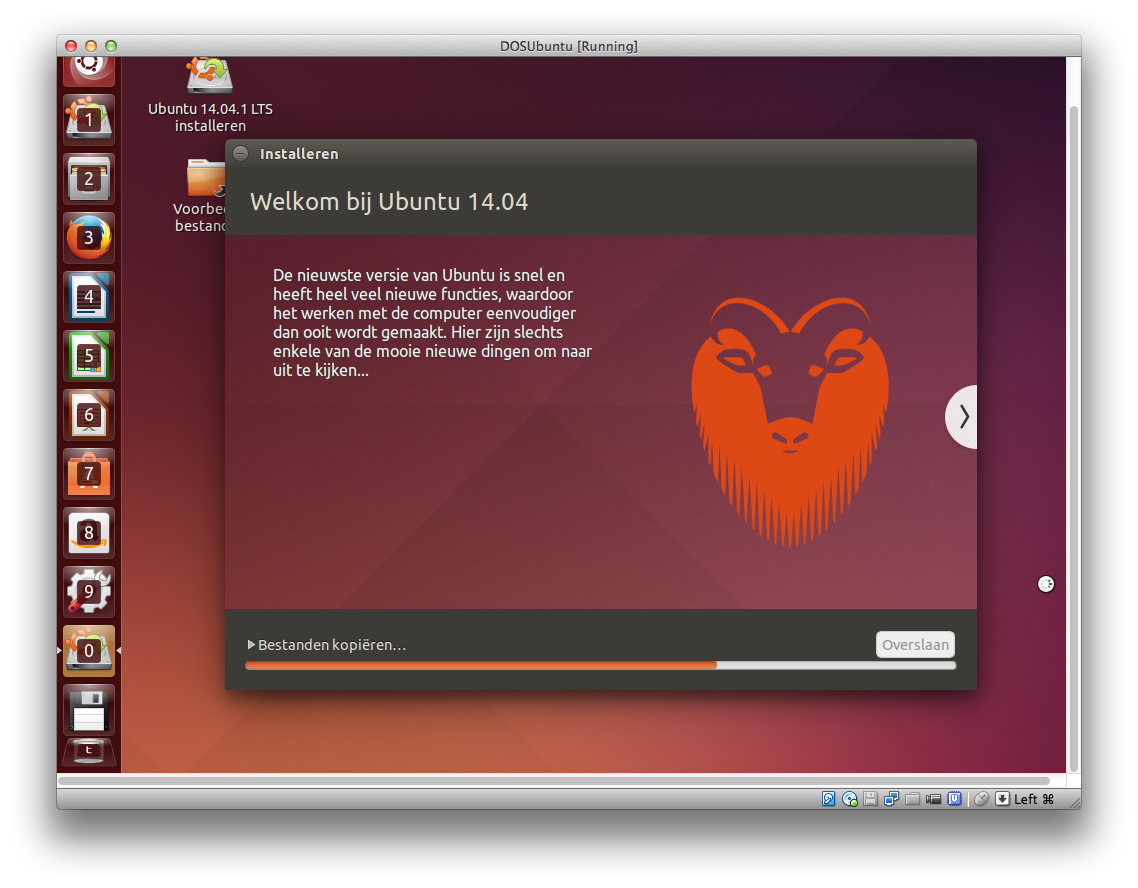
\includegraphics[width=\textwidth]{./IMG/R}
\end{figure}

\begin{figure}[H]
	\centering
	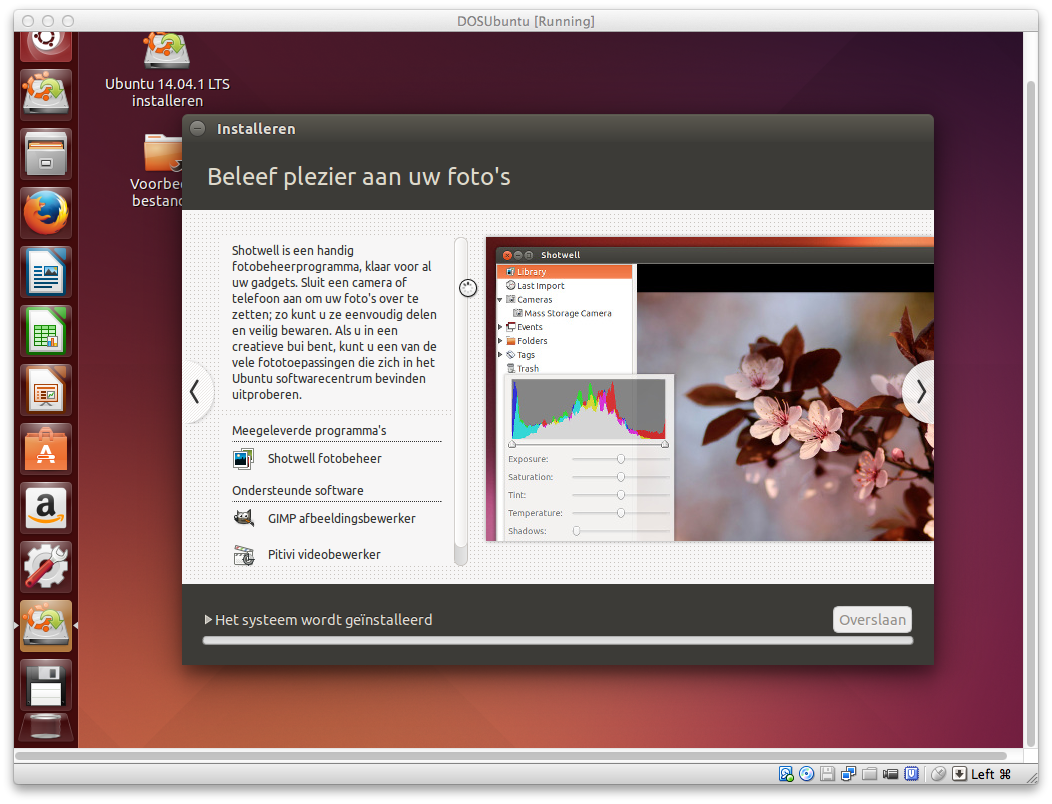
\includegraphics[width=\textwidth]{./IMG/S}
\end{figure}

Nu moet de VM herstarten:

\begin{figure}[H]
	\centering
	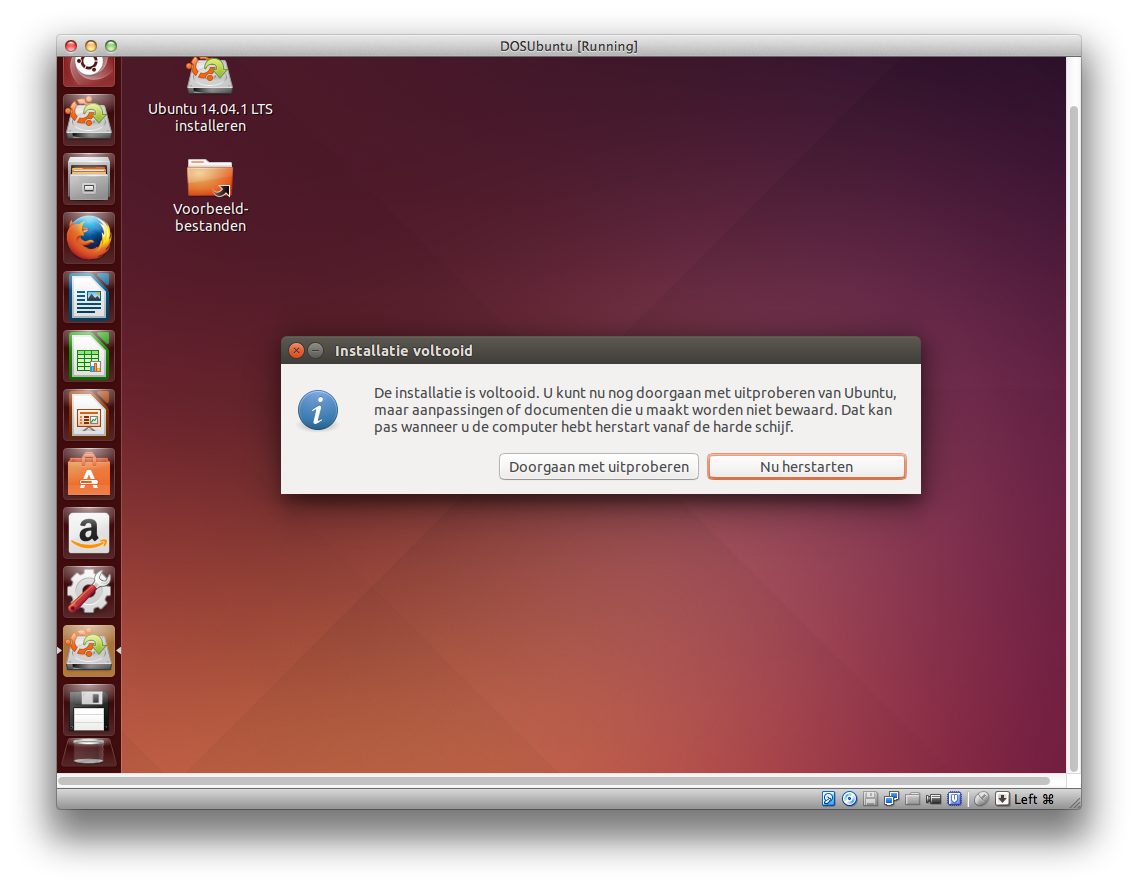
\includegraphics[width=\textwidth]{./IMG/T}
\end{figure}

Waarna de ISO uit de virtuele schijf verwijderd moet worden. 

\begin{figure}[H]
	\centering
	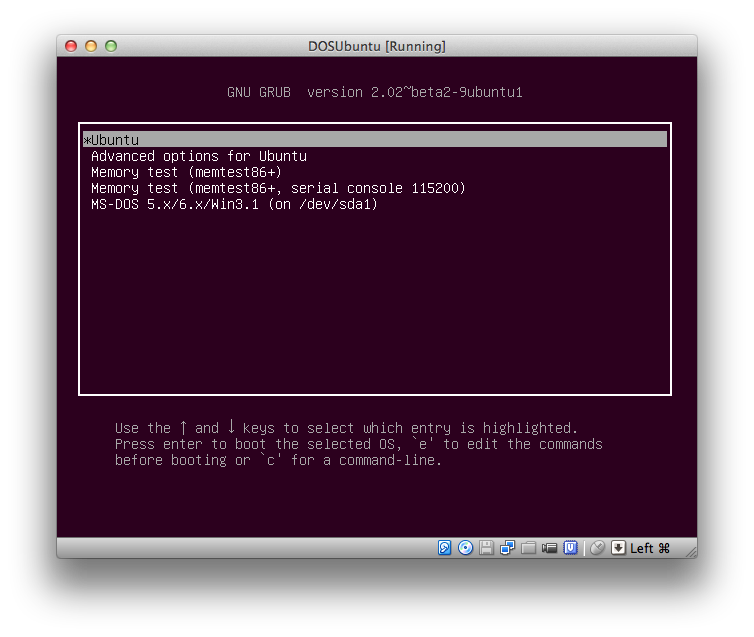
\includegraphics[width=\textwidth]{./IMG/V}
\end{figure}

De rest van de boot verloopt goed.

\begin{figure}[H]
	\centering
	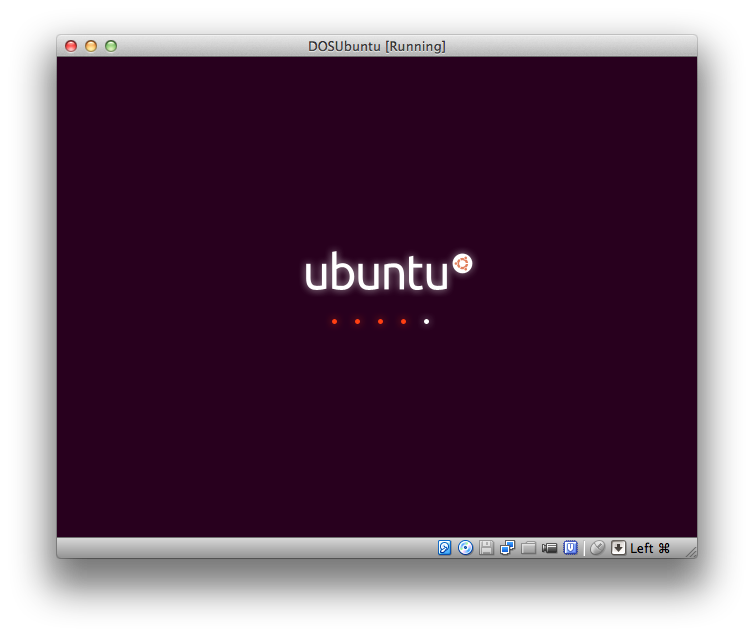
\includegraphics[width=\textwidth]{./IMG/W}
\end{figure}

\begin{figure}[H]
	\centering
	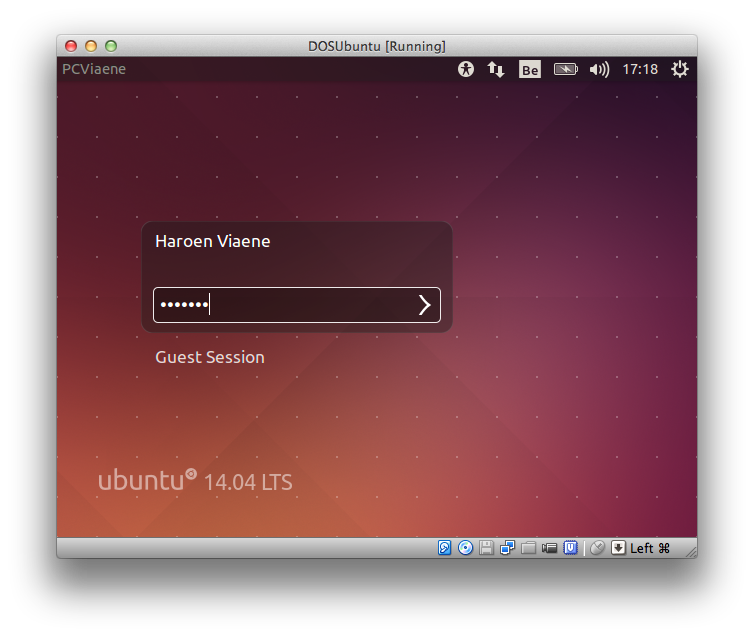
\includegraphics[width=\textwidth]{./IMG/X}
\end{figure}

\begin{figure}[H]
	\centering
	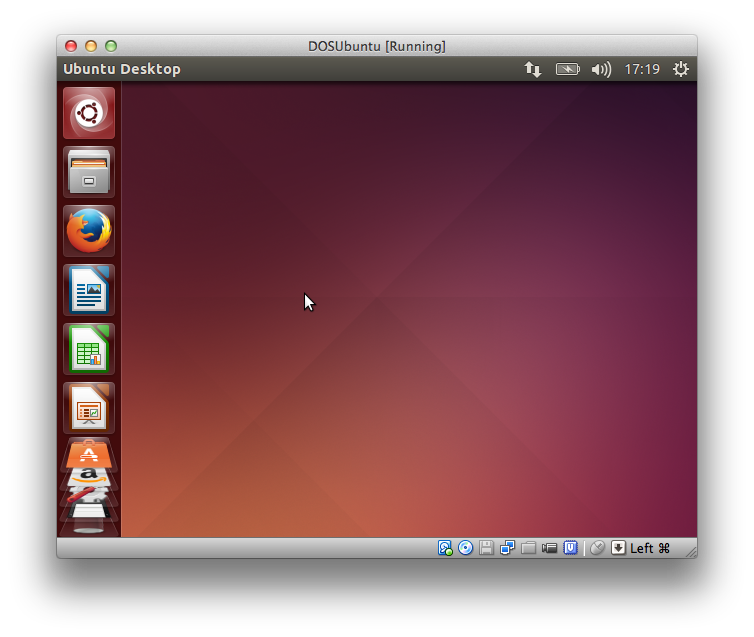
\includegraphics[width=\textwidth]{./IMG/Y}
\end{figure}

\section{Tijdens de installatie}

\begin{enumerate}
\item LTS betekent long term support. Bij Ubuntu is er elke twee jaar een nieuwe grote versie. Sinds Ubuntu 12.04 worden de grote versies 5 jaar ondersteund. Vroeger was Desktop 2 jaar en Server 5 jaar.
\item man ifconfig: 
	\begin{verbatim}IFCONFIG(8)               BSD System Manager's Manual              IFCONFIG(8)

NAME
     ifconfig -- configure network interface parameters

SYNOPSIS
     ifconfig [-L] [-m] [-r] interface [create] [address_family] [address
              [dest_address]] [parameters]
     ifconfig interface destroy
     ifconfig -a [-L] [-d] [-m] [-r] [-u] [-v] [address_family]
     ifconfig -l [-d] [-u] [address_family]
     ifconfig [-L] [-d] [-m] [-r] [-u] [-v] [-C]
     ifconfig interface vlan vlan-tag vlandev iface
	\end{verbatim}
\item main officially supported software, restricted is niet helemaal gratis software die wel volledig ondersteund is, universe is community maintained software, multiverse is betalende software
\item \begin{verbatim}sudo adduser <username> sudo\end{verbatim}
\end{enumerate}

\section{Uittesten}

Allereerst wordten de VirtualBox guest additions ge\"installeerd, zodat onder andere de schermresolutie in een iets verdraagbaare grootte is en de muis uit het venster kan gaan zonder van programma te wisselen. 

\begin{figure}[H]
	\centering
	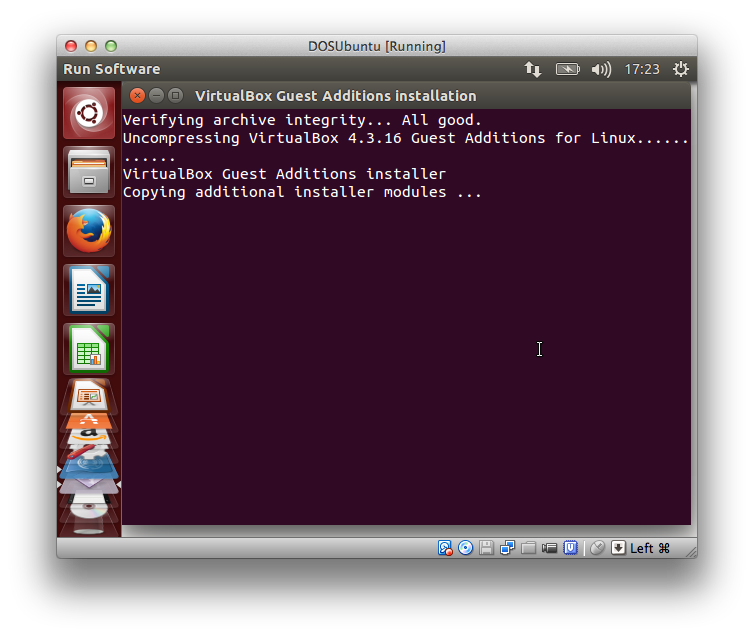
\includegraphics[width=\textwidth]{./IMG/Z}
	\caption{Installatie van de Guest Additions}
\end{figure}

Na een restart kunnen we nu echt beginnen. 

In een terminalvenster wordt mount ingevoerd: 

\begin{figure}[H]
	\centering
	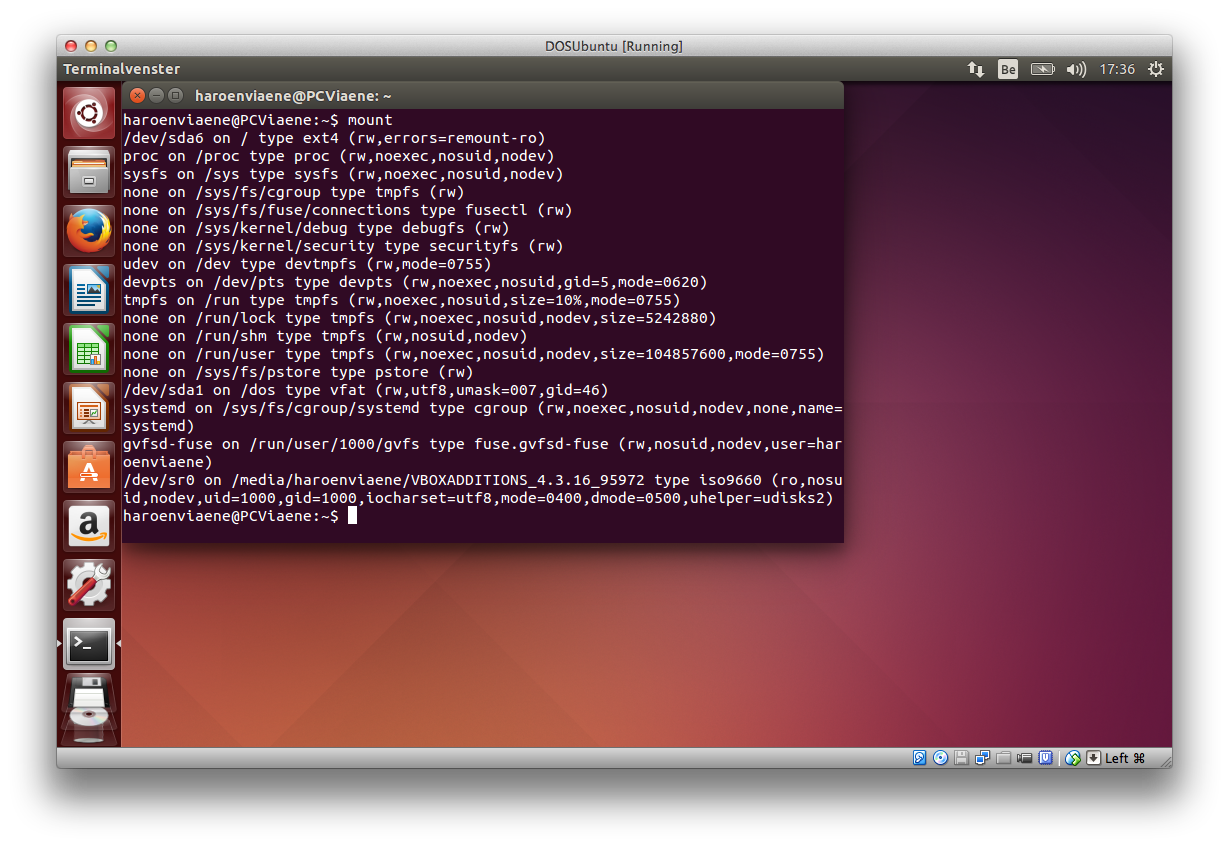
\includegraphics[width=\textwidth]{./IMG/ZA}
	\caption{mount}
\end{figure}

En daarna via openssh (die eerst ge\"installeerd werd) verbinding gemaakt met 127.0.0.1, waarna de cd-romdrive gekoppeld werd via VirtualBox, en dan ge-eject. 

\begin{figure}[H]
	\centering
	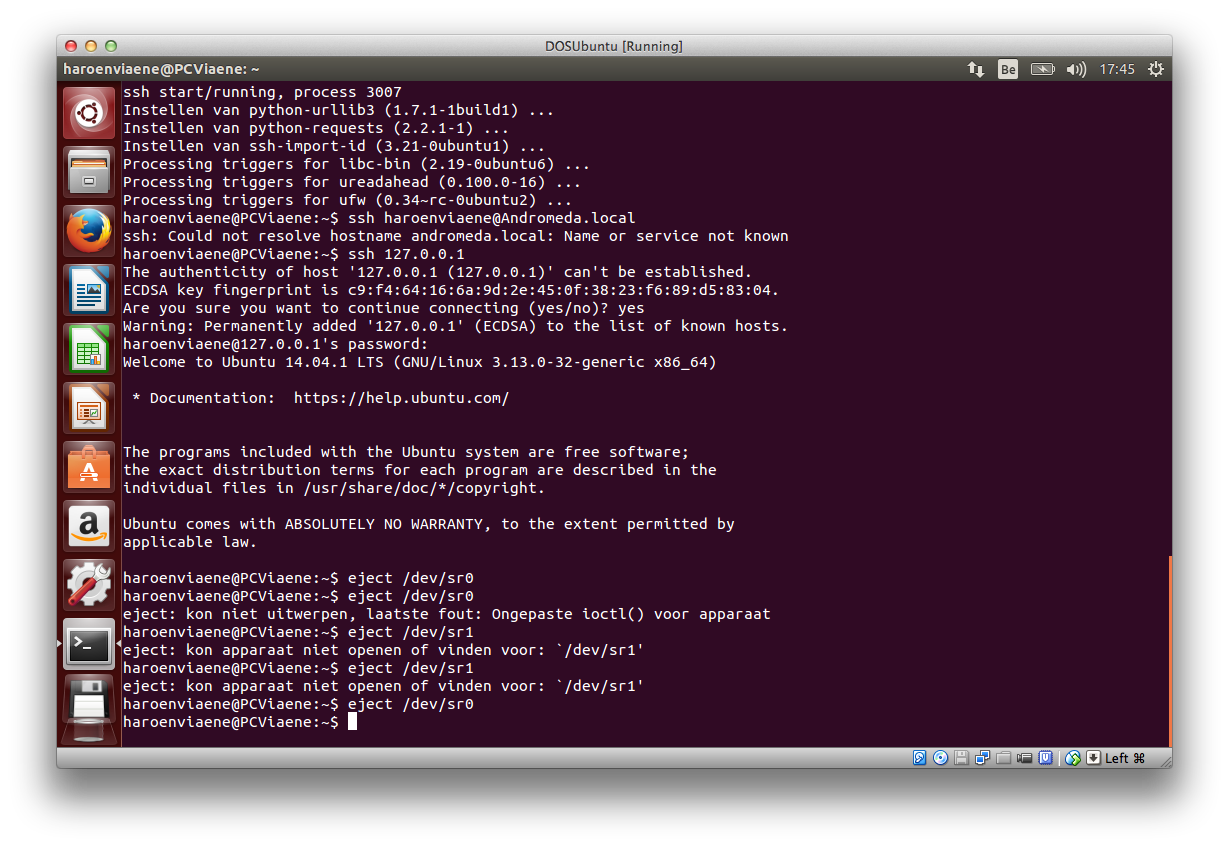
\includegraphics[width=\textwidth]{./IMG/ZB}
	\caption{Screenshot nadat de cd ge-eject was}
\end{figure}

Hierna werd de DOS aan het opstartmenu toegevoegd:

\begin{figure}[H]
	\centering
	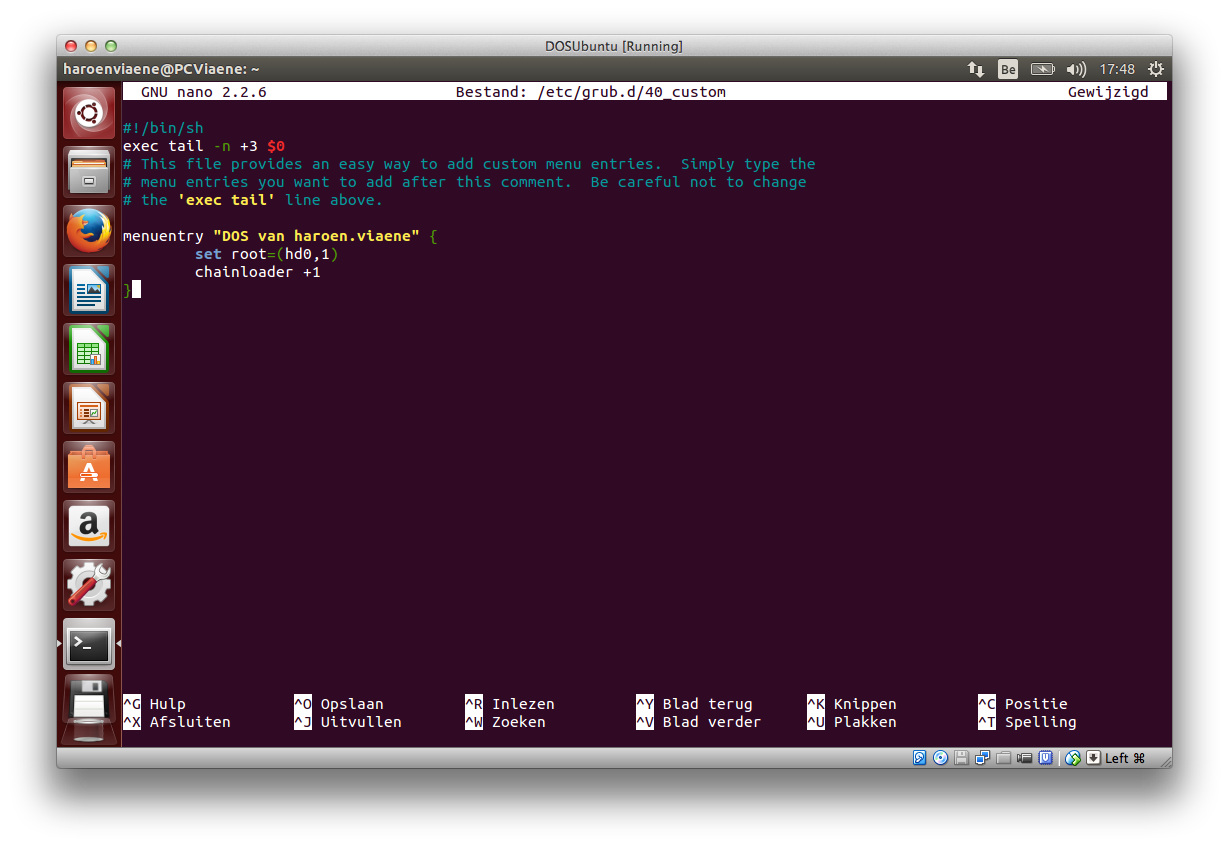
\includegraphics[width=\textwidth]{./IMG/ZC}
	\caption{40\_custom}
\end{figure}

\begin{figure}[H]
	\centering
	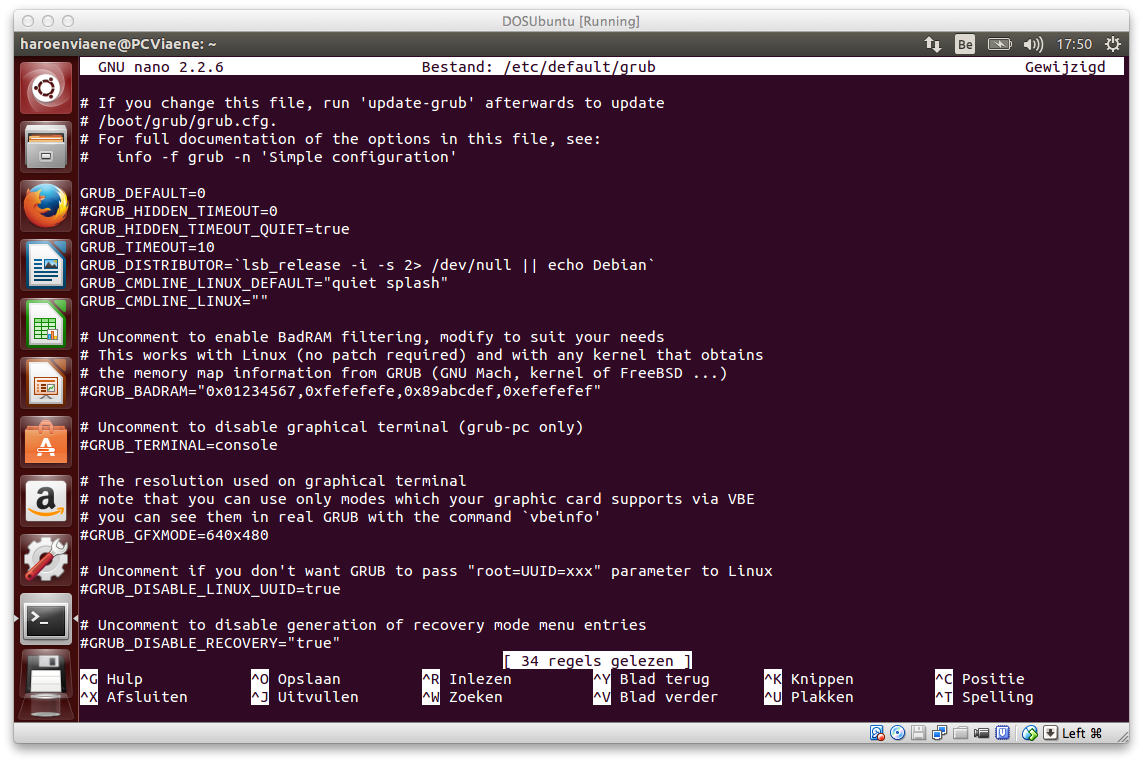
\includegraphics[width=\textwidth]{./IMG/ZD}
	\caption{grub}
\end{figure}

\begin{figure}[H]
	\centering
	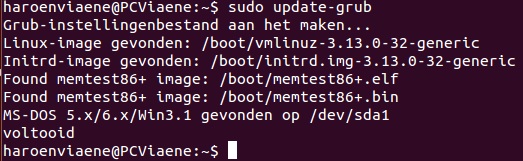
\includegraphics[width=\textwidth]{./IMG/ZE}
	\caption{grub-update}
\end{figure}

Daarna wordt DOS getest: 

\begin{figure}[H]
	\centering
	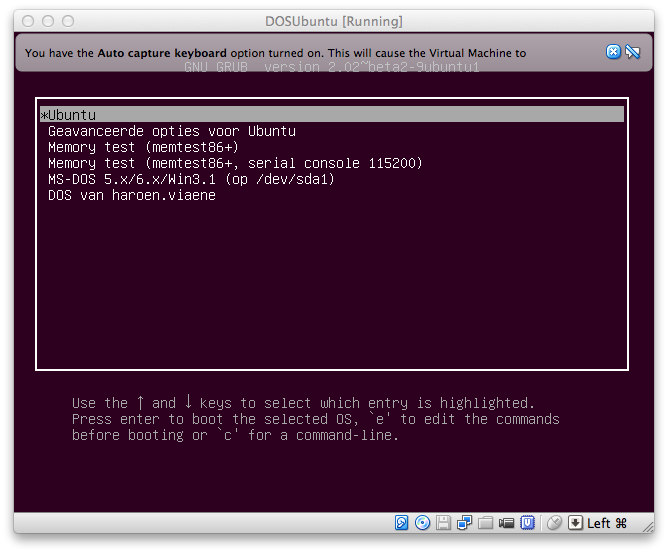
\includegraphics[width=\textwidth]{./IMG/ZF}
	\caption{boot-venster}
\end{figure}

\begin{figure}[H]
	\centering
	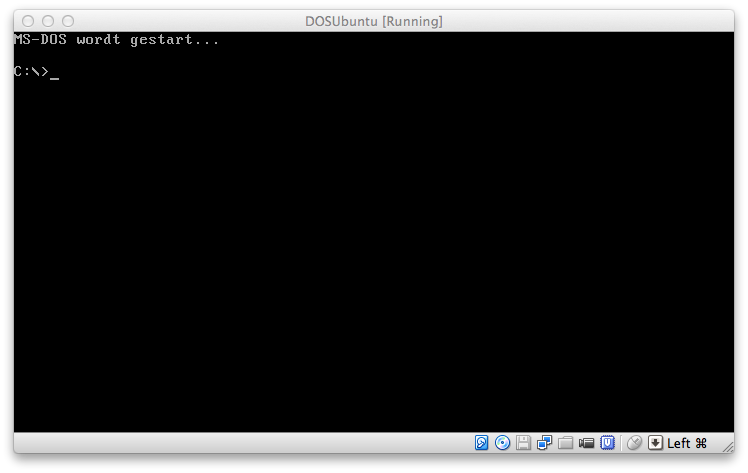
\includegraphics[width=\textwidth]{./IMG/ZG}
	\caption{DOS}
\end{figure}

\newpage











\end{document}